\RequirePackage[l2tabu, orthodox]{nag}
\RequirePackage{silence}
\documentclass[french,english]{beamer}
%INSTALL
\pdfgentounicode=1 %permits (with package glyphtounicode) to copy eg x ⪰ y iff v(x) ≥ v(y) from pdf to unicode data. 
\input{glyphtounicode}%TODO avoid warning when redefining → (and others) ; make it work for ℝ (U+211D) as well
\usepackage{lmodern}%has more characters such as ligatures, permit copy from resulting PDF. fntguide says to load the font before fontenc, to prevent default loading of cmr.
\usepackage[T1]{fontenc}%encode resulting accented characters correctly in resulting PDF, permits copy-paste
\usepackage[utf8]{inputenc}
\usepackage{newunicodechar}%able to use e.g. → or ≤ in source
\usepackage{textcomp}%useful for redefining → and ¬ and … (otherwise seems to attempt to use \textrightarrow and the like but are not defined)
% solves bug in lmodern, https://tex.stackexchange.com/a/261188/
\DeclareFontShape{OMX}{cmex}{m}{n}{
  <-7.5> cmex7
  <7.5-8.5> cmex8
  <8.5-9.5> cmex9
  <9.5-> cmex10
}{}

\SetSymbolFont{largesymbols}{normal}{OMX}{cmex}{m}{n}
\SetSymbolFont{largesymbols}{bold}  {OMX}{cmex}{m}{n}
%warn about missing characters
\tracinglostchars=2

%REDAC
\usepackage{lineno}
\usepackage{booktabs}
\usepackage{calc}
\usepackage{tabularx}

\usepackage{etoolbox} %for addtocmd, newtoggle commands
\newtoggle{LCpres}
\toggletrue{LCpres}

\usepackage{mathtools} %load this before babel!
	\mathtoolsset{showonlyrefs,showmanualtags}

\usepackage{natbib}%Package frenchb asks to load natbib before babel/frenchb
\usepackage{babel}%[french, english]: language options should be on the document level
%suppresses the warning about frenchb not modifying the captions (“—” to “:” in “Figure 1 – Legend”).
%	\frenchbsetup{AutoSpacePunctuation=false,SuppressWarning=true}% test with false?
	\frenchbsetup{AutoSpacePunctuation=false,SuppressWarning=false}

%\usepackage[super]{nth}%better use fmtcount! (loaded by datetime anyway; see below about pbl with warnings and package silence)
\usepackage{listings} %typeset source code listings
	\lstset{language=XML, tabsize=2, captionpos=b, basicstyle=\NoAutoSpacing}%NoAutoSpacing avoids space before colon or ?}%,literate={"}{{\tt"}}1, keywordstyle=\fontspec{Latin Modern Mono Light}\textbf, emph={String, PreparedStatement}, emphstyle=\fontspec{Latin Modern Mono Light}\textbf, language=Java, basicstyle=\small\NoAutoSpacing\ttfamily, frame=single, aboveskip=0pt, belowskip=0pt, showstringspaces=false
\usepackage[nolist,smaller,printonlyused]{acronym}%,smaller option produces warnings from relsize in some cases, it seems.% Note silence and acronym and hyperref make (xe)latex crash when ac used in section (http://tex.stackexchange.com/questions/103483/strange-packages-interaction-acronyms-silence-hyperref), rather use \section{\texorpdfstring{\acs{UE}}{UE}}.
\usepackage{fmtcount}
\usepackage[nodayofweek]{datetime}%must be loaded after the babel package. However, loading it after {nth} generates a warning from fmtcount about ordinal being already defined. Better load it before nth? (then we can remove the silence package which creates possible crashes, see above.) Or remove nth?  Also, with srcletter, problem: https://golatex.de/verwendung-von-babel-und-datetime-in-scrlttr2-schlaegt-fehlt-t14779.html. Possibly, use srcdate and srctime instead?
%\usepackage{xspace}%do we need this?
\nottoggle{LCpres}{
	\usepackage[textsize=small]{todonotes}
}{
}
\iftoggle{LCpres}{
	%remove pdfusetitle (implied by beamer)
	\usepackage{hyperref}
}{
% option pdfusetitle must be introduced here, not in hypersetup.
	\usepackage[pdfusetitle]{hyperref}
}
\nottoggle{LCpres}{
%seems like authblk wants to be later than hyperref, but sooner than silence
\usepackage{authblk}
\renewcommand\Affilfont{\small}
}{
}
\usepackage{silence}
\WarningFilter{newunicodechar}{Redefining Unicode character}
%breaklinks makes links on multiple lines into different PDF links to the same target.
%colorlinks (false): Colors the text of links and anchors. The colors chosen depend on the the type of link. In spite of colored boxes, the colored text remains when printing.
%linkcolor=black: this leaves other links in colors, e.g. refs in green, don't print well.
%pdfborder (0 0 1, set to 0 0 0 if colorlinks): width of PDF link border
%hidelinks or: colorlinks, linkcolor=black, citecolor=black, urlcolor={blue!80!black}
\hypersetup{breaklinks, bookmarksopen}
%add hyperfigures=true in hypersetup (already defined in article mode)
\iftoggle{LCpres}{
	\hypersetup{hyperfigures}
}{
}

%in Beamer, sets url colored links but does not change the rest of the colors (http://tex.stackexchange.com/questions/13423/how-to-change-the-color-of-href-links-for-real)
%\hypersetup{breaklinks,bookmarksopen,colorlinks=true,urlcolor=blue,linkcolor=,hyperfigures=true}
% hyperref doc says: Package bookmark replaces hyperref’s bookmark organization by a new algorithm (...) Therefore I recommend using this package.
\usepackage{bookmark}

% center floats by default, but do not use with float
% \usepackage{floatrow}
% \makeatletter
% \g@addto@macro\@floatboxreset\centering
% \makeatother
\nottoggle{LCpres}{
	\usepackage{enumitem} %follow enumerate by a string saying how to display enumeration
}{
}
\usepackage{ragged2e} %new com­mands \Cen­ter­ing, \RaggedLeft, and \RaggedRight and new en­vi­ron­ments Cen­ter, FlushLeft, and FlushRight, which set ragged text and are eas­ily con­fig­urable to al­low hy­phen­ation (the cor­re­spond­ing com­mands in LaTeX, all of whose names are lower-case, pre­vent hy­phen­ation al­to­gether). 
\usepackage{siunitx} %[expproduct=tighttimes, decimalsymbol=comma] ou (plus récent ?) [round-mode=figures, round-precision=2, scientific-notation = engineering]
\sisetup{detect-all, locale = FR, strict}% to detect e.g. when in math mode (use a math font) - check whether this makes sense with strict
\usepackage{braket} %for \Set
\usepackage{doi}

\usepackage{amsmath,amsthm}
\usepackage{amssymb}%for \mathbb{R} %includes amsfonts
\usepackage{bm}%“The \boldsymbol command is obtained preferably by using the bm package, which provides a newer, more powerful version than the one provided by the amsmath package. Generally speaking, it is ill-advised to apply \boldsymbol to more than one symbol at a time.” — AMS Short math guide. “If no bold font appears to be available for a particular symbol, \bm will use ‘poor man’s bold’” — bm
% \usepackage{dsfont} %for what?

\usepackage{environ}%for xdescwd command
%BUT see https://tex.stackexchange.com/questions/83798/cleveref-varioref-missing-endcsname-inserted for cleveref with french
\usepackage{cleveref}% cleveref should go "laster" than hyperref
%GRAPHICS
\usepackage{pgf}
\usepackage{pgfplots}
	\usetikzlibrary{babel, matrix, fit, plotmarks, calc, trees, shapes.geometric, positioning, plothandlers, arrows, shapes.multipart}
\pgfplotsset{compat=1.14}
\usepackage{graphicx}

\DeclareMathAlphabet\mathbfcal{OMS}{cmsy}{b}{n}

\graphicspath{{graphics/},{graphics-dm/}}
\DeclareGraphicsExtensions{.pdf}
\newcommand*{\IncludeGraphicsAux}[2]{%
	\XeTeXLinkBox{%
		\includegraphics#1{#2}%
	}%
}%

%HACKING
\usepackage{printlen}
\uselengthunit{mm}
% 	\newlength{\templ}% or LenTemp?
% 	\setlength{\templ}{6 pt}
% 	\printlength{\templ}
\usepackage{scrhack}% load at end. Corrects a bug in float package, which is outdated but might be used by other packages
\usepackage{mathrsfs}% for \mathscr
%see https://tex.stackexchange.com/questions/409212/size-substitution-with-fontsize-14
\DeclareFontFamily{U}{rsfs}{\skewchar\font127 }
\DeclareFontShape{U}{rsfs}{m}{n}{%
   <-6.5> rsfs5
   <6.5-8> rsfs7
   <8-> rsfs10
}{}

%Beamer-specific
%do not remove babel, which beamer uses (beamer uses the \translate command for the appendix); but french can be removed.
\iftoggle{LCpres}{
	\usepackage{appendixnumberbeamer}
	\setbeamertemplate{navigation symbols}{} 
	\usepackage{preamble/beamerthemeParisFrance}
	\usefonttheme{professionalfonts}
	\setcounter{tocdepth}{10}
	%From: http://tex.stackexchange.com/questions/168057/beamer-with-xelatex-on-texlive2013-enumerate-numbers-in-black
%I don’t think it’s useful to submit this as a bug: nothing has been solved since March, 2015. See: https://bitbucket.org/rivanvx/beamer/issues?status=resolved.

\setbeamertemplate{enumerate item}
{
  \begin{pgfpicture}{-1ex}{-0.65ex}{1ex}{1ex}
    \usebeamercolor[fg]{item projected}
    {\pgftransformscale{1.75}\pgftext{\normalsize\pgfuseshading{bigsphere}}}
    {\pgftransformshift{\pgfpoint{0pt}{0.5pt}}
      \pgftext{\usebeamercolor[fg]{item projected}\usebeamerfont*{item projected}\insertenumlabel}}
  \end{pgfpicture}%
}

\setbeamertemplate{enumerate subitem}
{
  \begin{pgfpicture}{-1ex}{-0.55ex}{1ex}{1ex}
    \usebeamercolor[fg]{subitem projected}
    {\pgftransformscale{1.4}\pgftext{\normalsize\pgfuseshading{bigsphere}}}
    \pgftext{%
      \usebeamercolor[fg]{subitem projected}%
      \usebeamerfont*{subitem projected}%
      \insertsubenumlabel}
  \end{pgfpicture}%
}

\setbeamertemplate{enumerate subsubitem}
{
  \begin{pgfpicture}{-1ex}{-0.55ex}{1ex}{1ex}
    \usebeamercolor[fg]{subsubitem projected}
    {\pgftransformscale{1.4}\pgftext{\normalsize\pgfuseshading{bigsphere}}}
    \pgftext{%
      \usebeamercolor[fg]{subsubitem projected}%
      \usebeamerfont*{subitem projected}%
      \insertsubsubenumlabel}
  \end{pgfpicture}%
}


}{
}
% \newcommand{\citep}{\cite}%Better: leave natbib.
% \setbeamersize{text margin left=0.1cm, text margin right=0.1cm} 
% \usetheme{BrusselsBelgium}%no, replace with paris
%\usetheme{ParisFrance}, no, usepackage better!
% Tex Gyre takes too much space, replace with Latin Modern Roman / Sans / Mono.
% Difference when loading explicitly Latin Modern Sans (compared to not using \setsansfont at all):
% the font LMSans17-Regular appears in the document;
% the title of the slides appears differently;
% it does not say (in the log file):
% > LaTeX Font Info:    Font shape `EU1/lmss/m/it' in size <10.95> not available
% > (Font)              Font shape `EU1/lmss/m/sl' tried instead on input line 85.
% > LaTeX Font Info:    Try loading font information for EU1+lmtt on input line 85.

%tikzposter-specific
%remove \usepackage{ragged2e}: causes 1=1 to be printed in the middle of the poster. (Anyway prints a warning about those characters being missing.)
%put [french, english] options next to \usepackage{babel} to avoid warning of 

\newcommand{\R}{ℝ}
\newcommand{\N}{ℕ}
\newcommand{\Z}{ℤ}
\newcommand{\card}[1]{\lvert{#1}\rvert}
\newcommand{\powerset}[1]{\mathscr{P}(#1)}%\mathscr rather than \mathcal: scr is rounder than cal (at least in XITS Math).
%powerset without zero
\newcommand{\powersetz}[1]{\mathscr{P}_\emptyset(#1)}
\newcommand{\suchthat}{\;\ifnum\currentgrouptype=16 \middle\fi|\;}
%\newcommand{\Rplus}{\reels^+\xspace}
%int interval, to be improved?
\newcommand{\intvl}[1]{\llbracket{}#1\rrbracket}
\DeclarePairedDelimiterX{\norm}[1]{\lVert}{\rVert}{#1}

\AtBeginDocument{%
	\renewcommand{\epsilon}{\varepsilon}
% we want straight form of \phi for mathematics, as recommended in UTR #25: Unicode support for mathematics.
%	\renewcommand{\phi}{\varphi}
}

% with amssymb, but I don’t want to use amssymb just for that.
% \newcommand{\restr}[2]{{#1}_{\restriction #2}}
%\newcommand{\restr}[2]{{#1\upharpoonright}_{#2}}
\newcommand{\restr}[2]{{#1|}_{#2}}%sometimes typed out incorrectly within \set.
%\newcommand{\restr}[2]{{#1}_{\vert #2}}%\vert errors when used within \Set and is typed out incorrectly within \set.
\DeclareMathOperator*{\argmax}{arg\,max}
\DeclareMathOperator*{\argmin}{arg\,min}


%Voting and MCDA
\newcommand{\allalts}{\mathscr{A}}
\newcommand{\alts}{A}
\newcommand{\allF}{\mathcal{F}}
\newcommand{\cat}[1]{C_{#1}}

%Voting
\newcommand{\feasalts}{F}
\newcommand{\allvoters}{\mathscr{N}}
\newcommand{\voters}{N}
\newcommand{\allsystems}{\mathcal{G}}
\newcommand{\prof}{\mathbf{R}}
\newcommand{\allprofs}{\mathbfcal{R}}
\newcommand{\linors}{\mathcal{L}(\alts)}

\newcommand{\pbasic}[1]{\prof^{#1}_\epsilon}
\newcommand{\pelem}[1]{\prof^{#1}_e}
\newcommand{\pcycl}[1]{\prof^{#1}_c}
\newcommand{\pcycllong}[1]{\prof^{#1}_{cl}}
\newcommand{\pinv}[1]{\overline{\prof_{#1}}}
\newcommand{\dmap}{{\xitsfamily δ}}

%logic atom
%⟼ (long)
\DeclareDocumentCommand{\lato}{ O{\prof} O{\alts} }{[#1 \!⟼\! #2]}
%logic atom in
%↝, \stackrel{\in}{\mapsto}, ➲, ⥹
\newcommand{\tightoverset}[2]{%
  \mathop{#2}\limits^{\vbox to -.5ex{\kern-0.9ex\hbox{$#1$}\vss}}}
\DeclareDocumentCommand{\latoin}{ O{\prof} O{\alpha} }{[#1 \tightoverset{\in}{⟼} #2]}
\newcommand{\alllang}{\mathcal{L}}
\newcommand{\ltru}{\texttt{T}}
\newcommand{\lfal}{\texttt{F}}
\newcommand{\laxiom}[1]{{\texgyreherosfamily{\textsc{#1}}}}

%ARG TH
\newcommand{\AF}{\mathcal{AF}}
\newcommand{\labelling}{\mathcal{L}}
\newcommand{\labin}{\textbf{in}\xspace}
\newcommand{\labout}{\textbf{out}}
\newcommand{\labund}{\textbf{undec}\xspace}
\newcommand{\nonemptyor}[2]{\ifthenelse{\equal{#1}{}}{#2}{#1}}
\newcommand{\gextlab}[2][]{
	\labelling{\mathcal{GE}}_{(#2, \nonemptyor{#1}{\ibeatsr{#2}})}
}
\newcommand{\allargs}{A^*}
\newcommand{\args}{A}
\newcommand{\ar}{a}
\newcommand{\ext}{\mathcal{E}}

%MCDA+Arg
\newcommand{\dm}{d}
\newcommand{\ileadsto}{\rightsquigarrow}
\newcommand{\mleadsto}[1][\eta]{\rightsquigarrow_{#1}}
\newcommand{\ibeats}{\vartriangleright}
\newcommand{\mbeats}[1][\eta]{\vartriangleright_{#1}}

%MISC
\newcommand{\lequiv}{\Vvdash}
\newcommand{\weightst}{W^{\,t}}

%MCDA classical
\newcommand{\crits}{\mathcal{J}}

%Sorting
\newcommand{\cats}{\mathcal{C}}
\newcommand{\catssubsets}{2^\cats}
\newcommand{\catgg}{\vartriangleright}
\newcommand{\catll}{\vartriangleleft}
\newcommand{\catleq}{\trianglelefteq}
\newcommand{\catgeq}{\trianglerighteq}
\newcommand{\alttoc}[2][x]{(#1 \xrightarrow{} #2)}
\newcommand{\alttocat}[3]{(#2 \xrightarrow{#1} #3)}
\newcommand{\alttoI}{(x \xrightarrow{} \left[\underline{C_x}, \overline{C_x}\right])}
\newcommand{\alttocatdm}[3][t]{\left(#2 \thinspace \raisebox{-3pt}{$\xrightarrow{#1}$}\thinspace #3\right)}
\newcommand{\alttocatatleast}[2]{\left(#1 \thinspace \raisebox{-3pt}{$\xrightarrow[]{≥}$}\thinspace #2\right)}
\newcommand{\alttocatatmost}[2]{\left(#1 \thinspace \raisebox{-3pt}{$\xrightarrow[]{≤}$}\thinspace #2\right)}

\definecolor{darkgreen}{rgb}{0,0.6,0}
\newcommand{\commentOC}[1]{{\small\color{blue}$\big[$OC: #1$\big]$}}
\newcommand{\commentOCf}[1]{{\small\color{blue}{\selectlanguage{french}$\big[$OC : #1$\big]$}}}
\newcommand{\commentYM}[1]{{\small\color{red}$\big[$YM: #1$\big]$}}
\newcommand{\commentYMf}[1]{{\small\color{red}{\selectlanguage{french}$\big[$YM : #1$\big]$}}}

\newcommand{\llabel}[1]{\hypertarget{lintarget:#1}{}\linelabel{lin:#1}}
\setlength\linenumbersep{9mm}
%then see https://tex.stackexchange.com/questions/428656/external-cross-reference-to-a-line-number-using-lineno-and-xr-hyper for referencing lines from another document

%this probably requires outdated float package, see doc KomaScript for an alternative.
% \newfloat{program}{t}{lop}
% \floatname{program}{PM}

%definition, theorem, lemma, example environments, qed trickery are only needed in article mode (not Beamer)
\nottoggle{LCpres}{
%style is plain by default (italic text)
	\newtheorem{definition}{Definition}
	\newtheorem{theorem}{Theorem}
%no italic: expected.
%http://tex.stackexchange.com/questions/144653/italicizing-of-amsthm-package
	\newtheorem{lemma}{Lemma}
%\crefname{axiom}{axiom}{axioms}%might be needed for workaround bug in cref when defining new theorems?

%\ifdefined\theorem\else
%\newtheorem{theorem}{\iflanguage{english}{Theorem}{Théorème}}
%\fi

\theoremstyle{remark}
	\newtheorem{examplex}{Example}
	\newtheorem{remarkx}{Remark}

%trickery allowing use of \qedhere and the like.
\newenvironment{example}{
	\pushQED{\qed}\renewcommand{\qedsymbol}{$\triangle$}\examplex
}{
	\popQED\endexamplex
}
\newenvironment{remark}{
	\pushQED{\qed}\renewcommand{\qedsymbol}{$\triangle$}\remarkx
}{
	\popQED\endremarkx
}
}{
}
\crefname{examplex}{example}{examples}% I wonder why this is unnecessary in case of singular

%which line breaks are chosen: accept worse lines, therefore reducing risk of overfull lines. Default = 200
\tolerance=2000
%accept overfull hbox up to...
\hfuzz=2cm
%reduces verbosity about the bad line breaks
\hbadness 5000
%reduces verbosity about the underful vboxes
\vbadness=1300
%sloppy sets tolerance to 9999
\apptocmd{\sloppy}{\hbadness 10000\relax}{}{}

\bibliographystyle{abbrvnat}
%or \bibliographystyle{apalike} for presentations?

%doi package uses old-style dx.doi url, see 3.8 DOI system Proxy Server technical details, “Users may resolve DOI names that are structured to use the DOI system Proxy Server (http://doi.org (preferred) or http://dx.doi.org).”, https://www.doi.org/doi_handbook/3_Resolution.html
\makeatletter
\patchcmd{\@doi}{dx.doi.org}{doi.org}{}{}
\makeatother

% WRITING
%\newcommand{\ie}{i.e.\@\xspace}%to try
%\newcommand{\eg}{e.g.\@\xspace}
%\newcommand{\etal}{et al.\@\xspace}
\newcommand{\ie}{i.e.\ }
\newcommand{\eg}{e.g.\ }
\newcommand{\mkkOK}{\checkmark}%\color{green}{\checkmark}
\newcommand{\mkkREQ}{\ding{53}}%requires pifont?%\color{green}{\checkmark}
\newcommand{\mkkNO}{}%\text{\color{red}{\textsf{X}}}

\newlength{\xdescwd}
\makeatletter
\NewEnviron{xdesc}{%
  \setbox0=\vbox{\hbadness=\@M \global\xdescwd=0pt
    \def\item[##1]{%
      \settowidth\@tempdima{\textbf{##1}:}%
      \ifdim\@tempdima>\xdescwd \global\xdescwd=\@tempdima\fi}
  \BODY}
  \begin{description}[leftmargin=\dimexpr\xdescwd+.5em\relax,
    labelindent=0pt,labelsep=.5em,
    labelwidth=\xdescwd,align=left]\BODY\end{description}}
\makeatother

\makeatletter
\newcommand{\boldor}[2]{%
	\ifnum\strcmp{\f@series}{bx}=\z@
		#1%
	\else
		#2%
	\fi
}
\newcommand{\textstyleElProm}[1]{\boldor{\MakeUppercase{#1}}{\textsc{#1}}}
\makeatother
\newcommand{\electre}{\textstyleElProm{Électre}\xspace}
\newcommand{\electreIv}{\textstyleElProm{Électre Iv}\xspace}
\newcommand{\electreIV}{\textstyleElProm{Électre IV}\xspace}
\newcommand{\electreIII}{\textstyleElProm{Électre III}\xspace}
\newcommand{\electreTRI}{\textstyleElProm{Électre Tri}\xspace}
% \newcommand{\utadis}{\texorpdfstring{\textstyleElProm{utadis}\xspace}{UTADIS}}
% \newcommand{\utadisI}{\texorpdfstring{\textstyleElProm{utadis i}\xspace}{UTADIS I}}

%TODO
% \newcommand{\textstyleElProm}[1]{{\rmfamily\textsc{#1}}} 

\newcommand{\llbracket}{\lbrack\!\lbrack}
\newcommand{\rrbracket}{\rbrack\!\rbrack}

\newunicodechar{ℕ}{\mathbb{N}}
\newunicodechar{ℝ}{\mathbb{R}}
\newunicodechar{−}{\ifmmode{-}\else\textminus\fi}
\newunicodechar{≠}{\ensuremath{\neq}}
\newunicodechar{≤}{\ensuremath{\leq}}
\newunicodechar{≥}{\ensuremath{\geq}}
\newunicodechar{≻}{\succ}
\newunicodechar{⊁}{\nsucc}
\newunicodechar{⪰}{\succeq}
\newunicodechar{▷}{\triangleright}
\newunicodechar{⋫}{\ntriangleright}
\newunicodechar{→}{\ifmmode\rightarrow\else\textrightarrow\fi}
\newunicodechar{⟼}{\ifmmode\longmapsto\else\textlongmapsto\fi}%untested
\newunicodechar{⇒}{\ensuremath{\Rightarrow}}
\newunicodechar{⇏}{\ensuremath{\nRightarrow}}
\newunicodechar{⇔}{\ensuremath{\Leftrightarrow}}
\newunicodechar{∪}{\cup}
\newunicodechar{∩}{\cap}
\newunicodechar{∧}{\land}
\newunicodechar{∨}{\lor}
\newunicodechar{¬}{\ifmmode\lnot\else\textlnot\fi}
\newunicodechar{…}{\ifmmode\ldots\else\textellipsis\fi}
\newunicodechar{×}{\ifmmode\times\else\texttimes\fi}
\newunicodechar{γ}{\ensuremath{\gamma}}
\newunicodechar{δ}{\ensuremath{\delta}}
\newunicodechar{□}{\Box}


%const
\newcommand{\tikzboxit}{\path node[draw, overlay, inner sep=0.6mm, fit=(boxed), rectangle] {};}%

\newlength{\GraphsNodeSep}
\setlength{\GraphsNodeSep}{7mm}

% MCDA Drawing Sorting
\newlength{\MCDSCatHeight}
\setlength{\MCDSCatHeight}{6mm}
\newlength{\MCDSAltHeight}
\setlength{\MCDSAltHeight}{4mm}
%separation between two vertical alts
\newlength{\MCDSAltSep}
\setlength{\MCDSAltSep}{2mm}
\newlength{\MCDSCatWidth}
\setlength{\MCDSCatWidth}{3cm}
\newlength{\MCDSAltWidth}
\setlength{\MCDSAltWidth}{2.5cm}
\newlength{\MCDSEvalRowHeight}
\setlength{\MCDSEvalRowHeight}{6mm}
\newlength{\MCDSAltsToCatsSep}
\setlength{\MCDSAltsToCatsSep}{1.5cm}
\newcounter{MCDSNbAlts}
\newcounter{MCDSNbCats}
\newlength{\MCDSArrowDownOffset}
\setlength{\MCDSArrowDownOffset}{0mm}

\tikzset{/Graphs/dot/.style={
	shape=circle, fill=black, inner sep=0, minimum size=1mm
}}
\tikzset{/MC/D/S/alt/.style={
	shape=rectangle, draw=black, inner sep=0, minimum height=\MCDSAltHeight, minimum width=\MCDSAltWidth
}}
\tikzset{MC/D/S/pref/.style={
	shape=ellipse, draw=gray, thick
}}
\tikzset{/MC/D/S/cat/.style={
	shape=rectangle, draw=black, inner sep=0, minimum height=\MCDSCatHeight, minimum width=\MCDSCatWidth
}}
\tikzset{/MC/D/S/evals matrix/.style={
	matrix, row sep=-\pgflinewidth, column sep=-\pgflinewidth, nodes={shape=rectangle, draw=black, inner sep=0mm, text depth=0.5ex, text height=1em, minimum height=\MCDSEvalRowHeight, minimum width=12mm}, nodes in empty cells, matrix of nodes, inner sep=0mm, outer sep=0mm, row 1/.style={nodes={draw=none, minimum height=0em, text height=, inner ysep=1mm}}
}}

\newlength{\GitCommitSep}
\setlength{\GitCommitSep}{13mm}

\tikzset{/Git/commit/.style={
	shape=rectangle, draw, minimum width=4em, minimum height=0.6cm
}}
\tikzset{/Git/branch/.style={
	shape=ellipse, draw, red
}}
\tikzset{/Git/head/.style={
	shape=ellipse, draw, fill=yellow
}}

\tikzset{profile matrix/.style={
	matrix of math nodes, column sep=3mm, row sep=2mm, nodes={inner sep=0.5mm, anchor=base}
}}
\tikzset{rank-profile matrix/.style={
	matrix of math nodes, column sep=3mm, row sep=2mm, nodes={anchor=base}, column 1/.style={nodes={inner sep=0.5mm}}, row 1/.style={nodes={inner sep=0.5mm}}
}}
\tikzset{rank-vector/.style={
	draw, rectangle, inner sep=0, outer sep=1mm
}}
\tikzset{isolated rank-vector/.style={
	draw, matrix of math nodes, column sep=3mm, inner sep=0, matrix anchor=base, nodes={anchor=base, inner sep=.33em}, ampersand replacement=\&
}}

% GUI
\tikzset{/GUI/button/.style={
	rectangle, very thick, rounded corners, draw=black, fill=black!40%, top color=black!70, bottom color=white
}}

% Logger objects
\tikzset{/logger/main/.style={
	shape=rectangle, draw=black, inner sep=1ex, minimum height=7mm
}}
\tikzset{/logger/helper/.style={
	shape=rectangle, draw=black, dashed, minimum height=7mm
}}
\tikzset{/logger/helper line/.style={
	<->, draw, dotted
}}

% Beliefs
\tikzset{/Beliefs/D/S/attacker/.style={
	shape=rectangle, draw, minimum size=8mm
}}
\tikzset{/Beliefs/D/S/supporter/.style={
	shape=circle, draw
}}

\newcommand{\tikzmark}[1]{%
	\tikz[overlay, remember picture, baseline=(#1.base)] \node (#1) {};%
}


\begin{acronym}
\acro{AMCD}{Aide Multicritère à la Décision}
\acro{ASA}{Argument Strength Assessment}
\acro{DA}{Decision Analysis}
\acro{DM}{Decision Maker}
\acro{DPr}{Deliberated Preferences}
\acro{DRSA}{Dominance-based Rough Set Approach}
\acro{DSS}{Decision Support Systems}
\acrodefplural{DSS}{Decision Support Systems}
% \newacroplural{DSS}[DSSes]{Decision Support Systems}
\acro{EJOR}{European Journal of Operational Research}
\acro{LNCS}{Lecture Notes in Computer Science}
\acro{MCDA}{Multicriteria Decision Aid}
\acro{MIP}{Mixed Integer Program}
\acro{NCSM}{Non Compensatory Sorting Model}
\acro{PL}{Programme Linéaire}
\acro{PLNE}{Programme Linéaire en Nombres Entiers}
\acro{PM}{Programme Mathématique}
\acro{MP}{Mathematical Program}
\acro{MIP}{Mixed Integer Program}
% \newacroplural{PM}{Programmes Mathématiques}
%acrodefplural since version 1.35, my debian has \ProvidesPackage{acronym}[2009/01/25, v1.34, Support for acronyms (Tobias Oetiker)]
\acrodefplural{PM}{Programmes Mathématiques}
\acro{PMML}{Predictive Model Markup Language}
\acro{RESS}{Reliability Engineering \& System Safety}
\acro{SMAA}{Stochastic Multicriteria Acceptability Analysis}
\acro{URPDM}{Uncertainty and Robustness in Planning and Decision Making}
\acro{XML}{Extensible Markup Language}
\end{acronym}


%\setbeamertemplate{headline}[singleline]
%\setbeamertemplate{footline}[authortitle]

\title[Automatic argumentation]{Towards automatic argumentation about voting rules}
\subject{Social choice}
\keywords{empirical, theorem proving, automatic proofs}
\author{Michael Kirsten \inst{1} \and \emph{Olivier Cailloux} \inst{2}}
\institute[KIT, LAMSADE]{\inst{1} Dept. of Informatics, Karlsruhe Institute of Technology (KIT) \and \inst{2} LAMSADE, Université Paris-Dauphine}
\date{\formatdate{3}{7}{2018}}

\begin{document}
\begin{frame}[plain]
	\tikz[remember picture,overlay]{
		\path (current page.south west) node[anchor=south west, inner sep=0] {
			
\includegraphics[height=1cm]{LAMSADE95.jpg}
		};
		\path (current page.south) ++ (0, 1mm) node[anchor=south, inner sep=0] {
			
\includegraphics[height=9mm]{Dauphine.jpg}
		};
		\path (current page.south east) node[anchor=south east, inner sep=0] {
			
\includegraphics[height=1cm]{PSL.png}
		};
		\path (current page.south) ++ (0, 4em) node[anchor=south, inner sep=0] {
			\scriptsize\url{https://github.com/oliviercailloux/voting-rule-argumentation-pres}
		};
%thanks to https://stackoverflow.com/questions/2423777/is-it-possible-to-create-a-remote-repo-on-github-from-the-cli-without-opening-br/13366414#13366414
%curl -u 'oliviercailloux' https://api.github.com/user/repos -d '{"name":"voting-rule-argumentation-pres"}'
%git remote add origin git@github.com:oliviercailloux/voting-rule-argumentation-pres.git
%git push --set-upstream origin master
	}
	\titlepage
\end{frame}
\addtocounter{framenumber}{-1}

\begin{frame}
	\frametitle{Introduction}
	\begin{block}{Context}
	\begin{itemize}
		\item Voting rule: a systematic way of aggregating different opinions and decide
		\item Multiple reasonable ways of doing this
		\item Different voting rules have different interesting properties
		\item None satisfy all desirable properties
	\end{itemize}
	\end{block}
	\begin{block}{Our goal}
		We want to easily communicate about strength and weaknesses of voting rules.
	\end{block}
\end{frame}

\begin{frame}
	\frametitle{Outline}
	\tableofcontents[hideallsubsections, sectionstyle=shaded/show]
\end{frame}

\AtBeginSection{
	\begin{frame}
		\frametitle{Outline}
		\tableofcontents[currentsection, hideallsubsections]
	\end{frame}
}

\section{Context}
\subsection{Introduction}
\begin{frame}[fragile]
	\frametitle{Voting rule}
	
	\begin{description}[Profile (on $A$)]
		\item[Alternatives] $\allalts = \set{a, b, c, d, \ldots}$; $\card{\allalts}=m$
		\item[Possible voters] $\allvoters = \set{1, 2, \ldots}$
		\item[Voters] $\emptyset \subset \voters \subseteq \allvoters$
%		\item[Linear orders on $A \subseteq \allalts$] $\linors$.
		\item[Profile] partial function $\prof$ from $\allvoters$ to linear orders on $\allalts$.
		\item[Voting rule] function $f$ mapping each $\prof$ to winners $\emptyset \subset A \subseteq \allalts$.
	\end{description}
	\vfill
	\begin{center}
		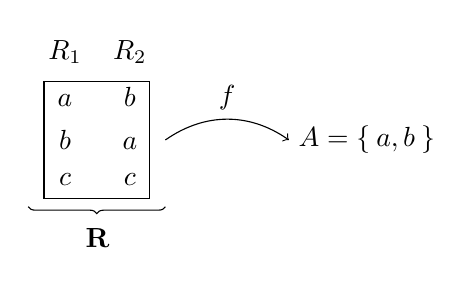
\begin{tikzpicture}
			\path node[profile matrix] (profile) {
				R_1&
				R_2
				\\
				| (profile11) | a&
				b
				\\
				b&
				a
				\\
				c&
				| (profile32) | c
				\\
			};
			\path ($(profile.south west)!.5!(profile.south east)$) ++ (0, -5mm) node {$\prof$};
			
			\path node[draw, rectangle, fit=(profile11) (profile32), outer xsep=2mm, outer ysep=1mm] (justprofile) {};
			\path (justprofile.east) ++ (2.5cm, 0) node[inner sep=0] (winners) {\mbox{} $A = \Set{a, b}$};
			\path[draw, ->] (justprofile.east) to[bend left=35] node[anchor=south] {$f$} (winners.west);

			\path[draw, decorate, decoration={brace, mirror}] (justprofile.south west) -- (justprofile.south east);
		\end{tikzpicture}
	\end{center}
\end{frame}

\begin{frame}[fragile]
	\frametitle{Example profile}
	\begin{equation}
		\begin{array}{lrrrrrr}
			&\multicolumn{6}{c}{\text{nb voters}}\\
		\cmidrule{2-7}
				&33	&16	&3	&8	&18	&22	\\
		\midrule
			1	&a	&b	&c	&c	&d	&e	\\
			2	&b	&d	&d	&e	&e	&c	\\
			3	&c	&c	&b	&b	&c	&b	\\
			4	&d	&e	&a	&d	&b	&d	\\
			5	&e	&a	&e	&a	&a	&a	\\
		\end{array}
	\end{equation}
	Who wins?\pause
	\begin{itemize}
		\item Most top-1: $a$
		\item $c$ is in the top 3 for everybody
		\item delete worst first, lowest nb of pref: $c$, $b$, $e$, $a$ ⇒ $d$
		\item delete worst first, from bottom: $a$, $e$, $d$, $b$ ⇒ $c$
		\item Borda: $b$
%		\item Condorcet: $c$
	\end{itemize}
\end{frame}

\subsection{Two voting rules}
\begin{frame}
	\frametitle{Borda}
	Given a profile $\prof$:
	\begin{itemize}
		\item score of $a \in \allalts$: number of alternatives it beats
		\item the highest scores win
	\end{itemize}
	
	\begin{equation}
		\prof =
		\begin{array}{rrrrr}
			a	&	a	&	a	&	b	&	b\\
			b	&	b	&	b	&	c	&	c\\
			c	&	c	&	c	&	a	&	a
		\end{array}
	\end{equation}
	\begin{itemize}
		\item score $a$ is\dots? \pause $2 + 2 + 2 = 6$
		\item score $b$ is $1 + 1 + 1 + 2 + 2 = 7$
		\item score $c$ is $1 + 1 = 2$
	\end{itemize}
	Winner: $b$.
\end{frame}

\begin{frame}
	\frametitle{Copeland}
	Given a profile $\prof$:
	\begin{itemize}
		\item score of $a \in \allalts$: number of alternatives against which it obtains a strict majority…
		\item … minus: number of alternatives that obtains a strict majority against $a$
		\item the highest scores win
	\end{itemize}
	
	
	\begin{equation}
		\prof =
		\begin{array}{rrrrr}
			a	&	a	&	a	&	b	&	b\\
			b	&	b	&	b	&	c	&	c\\
			c	&	c	&	c	&	a	&	a
		\end{array}
	\end{equation}
	\begin{itemize}
		\item score $a$ is\dots? \pause $\card{\set{b, c}} - \card{\emptyset} = 2$
		\item score $b$ is $\card{\set{c}} - \card{\set{a}} = 0$
		\item score $c$ is $\card{\emptyset} - \card{\set{a, b}} = -2$
	\end{itemize}
	Winner: $a$.
\end{frame}
	
\subsection{Axiomatic analysis}
\begin{frame}
	\frametitle{\subsecname}
	\begin{quote}
		Rather than dream up a multitude of arbitration schemes and determine whether or not each withstands the best of plausibility in a host of special cases, let us invert the procedure. Let us examine our subjective intuition of fairness and formulate this as a set of precise desiderata that any acceptable arbitration scheme must fulfil. Once these desiderata are formalized as axioms, then the problem is reduced to a mathematical investigation of the existence of and characterization of arbitration schemes which satisfy the axioms.
	\end{quote}
	\citet[p. 121]{luce_games_1957}\par
\end{frame}

\begin{frame}
	\frametitle{What’s an axiom?}
	\begin{itemize}
		\item An axiom (for us) is a principle
		\item Expressed formally
		\item That dictates some behavior of a voting rule
		\item In some conditions
		\item Usually seen as something to be satisfied
		\item Ideally, some union of some such axioms define exactly one rule
		\item Some axioms can be shown to be incompatible
	\end{itemize}
\end{frame}

\begin{frame}
	\frametitle{Unanimity}
	\begin{definition}[Unanimity]
		We ought to select as winner someone who has no unanimously preferred alternative
	\end{definition}
	\begin{equation}
		\prof =
		\begin{array}{rrr}
			a	&	a	&	b\\
			b	&	b	&	c\\
			c	&	c	&	a
		\end{array}
	\end{equation}
	Constraint? \pause Do not take $c$ as $b$ is unanimously preferred to it.	\pause
	\begin{equation}
		\prof =
		\begin{array}{rrr}
			a	&	a	&	b\\
			b	&	c	&	c\\
			c	&	b	&	a
		\end{array}
	\end{equation}
	Constraint? \pause No constraint.
\end{frame}

\begin{frame}
	\frametitle{Condorcet’s principle}
	\begin{block}{Condorcet’s principle}
		We ought to take the Condorcet winner as sole winner if it exists.
		\begin{itemize}
			\item $a$ \emph{beats} $b$ iff more than half the voters prefer $a$ to $b$.
			\item $a$ is a \emph{Condorcet winner} iff $a$ beats every other alternatives.
		\end{itemize}
	\end{block}
	\vfill
	\begin{equation}
		\prof =
		\begin{array}{rrrrr}
			a	&	a	&	a	&	b	&	b\\
			b	&	b	&	b	&	c	&	c\\
			c	&	c	&	c	&	a	&	a
		\end{array}
	\end{equation}
	 Who wins? \pause $a$
\end{frame}

\begin{frame}
	\frametitle{Borda does not satisfy Condorcet}
	\begin{equation}
		\prof =
		\begin{array}{rrrrr}
			a	&	a	&	a	&	b	&	b\\
			b	&	b	&	b	&	c	&	c\\
			c	&	c	&	c	&	a	&	a
		\end{array}
	\end{equation}
	\begin{itemize}
		\item Borda winners? \pause $b$
		\item Condorcet winner? \pause $a$
	\end{itemize}
\end{frame}

\begin{frame}
	\frametitle{Cancellation}
	\begin{definition}[Cancellation]
		When all pairs of alternatives $(a, b)$ in a profile are such that $a$ is preferred to $b$ as many times as $b$ to $a$, we ought to select all winners as ex-æquo
	\end{definition}
	\begin{example}
		\begin{equation}
			f\left(%
			\begin{array}{rrrr}
				a&b&c&c\\
				b&a&a&b\\
				c&c&b&a\\
			\end{array}\right) = \allalts
		\end{equation}
	\end{example}
\end{frame}

\begin{frame}
	\frametitle{Reinforcement}
	\begin{definition}[Reinforcement]
		When joining two sets of voters, exactly those winners that each set accepts should be selected, if possible
	\end{definition}
	\begin{example}
		\begin{equation}
			\prof_1 =
			\begin{array}{cc}
				a&b\\
				b&a\\
				c&c\\
			\end{array},
			A_1 = \set{a, b},
			\prof_2 =
			\begin{array}{ccc}
				a&b&a\\
				b&a&c\\
				c&c&b\\
			\end{array},
			A_2 = \set{a},
		\end{equation}
		\begin{equation}
			\prof =
			\begin{array}{ccccc}
				a&b&a&b&a\\
				b&a&b&a&c\\
				c&c&c&c&b\\
			\end{array}.
			\text{ Winners? }
			\pause
			\set{a}
		\end{equation}
	\end{example}
\end{frame}

\subsection{Objective}
\begin{frame}
	\frametitle{Our objective}
	Produce automatically “arguments” of the kind: voting rule $f$ does not satisfy axiom $a$
	\begin{itemize}
		\item To better understand their differences
		\item To help debate and choose a voting rule
		\item To investigate empirical attitudes towards given voting rules
	\end{itemize}
\end{frame}

\section{Approach}
\subsection{Software Bounded Model Checking}
\begin{frame}[fragile]{Software Bounded Model Checking (SBMC)}
\hspace*{-1em}
\begin{minipage}{0.5\textwidth}
\begin{block}{}
\vspace*{-1em}
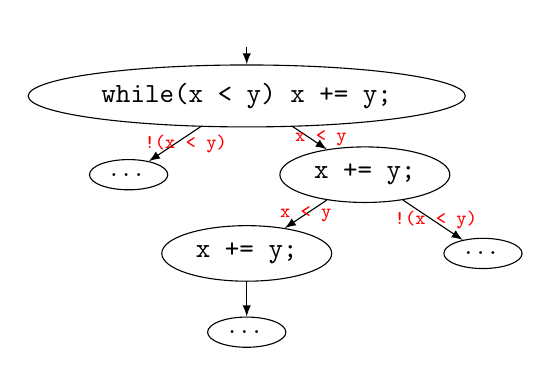
\begin{tikzpicture}
{%\footnotesize
\node (before) at (0,5.75) {};
\node[ellipse, draw] (start) at (0,5) {\texttt{while(x < y) x += y;}};
\node[ellipse, draw] (threea) at (-1.5,4) {\dots};
\node[ellipse, draw] (threeb) at (1.5,4) {\texttt{x += y;}};
\node[ellipse, draw] (fivea) at (0,3) {\texttt{x += y;}};
\node[ellipse, draw] (fiveb) at (3,3) {\dots};
\node[ellipse, draw] (seven) at (0,2) {\dots};
}
{\scriptsize
\path[-latex,draw] (start) -- (threea) node [midway,red] {\quad\texttt{\textbf{!(x < y)}}};
\path[-latex,draw] (start) -- (threeb) node [midway,red] {\quad\texttt{\textbf{x < y}}};

\path[-latex,draw] (threeb) -- (fivea) node [midway,red] {\texttt{\textbf{x < y}}};
\path[-latex,draw] (threeb) -- (fiveb) node [midway,red] {\;\texttt{\textbf{!(x < y)}}};
}

{\normalsize
\path[-latex,draw] (fivea) -- (seven);
\path[-latex,draw] (before) -- (start);
}
\end{tikzpicture}
\end{block}
\end{minipage}\begin{minipage}{0.55\textwidth}
\begin{itemize}
\item Static program analysis using symbolic execution
\item Exhaustive check by unwinding\\ the control flow graph
\item Bounded in number of loop unwindings and recursions
\end{itemize}
\end{minipage}

\pause
\begin{itemize}
\item SBMC tool converts program into logical equations, sent to SAT solver
\item Special “unwinding assertion” claims added to check whether longer program paths may be possible
\item Checks whether specified assertions can be violated
\end{itemize}
\end{frame}

\begin{frame}{Specifying and Verifying Properties in SBMC\hspace*{-1.8em}}
\begin{block}{Specification}
\begin{itemize}
%\item Program automatically encoded into logic using SSA form
\item Properties specified using \texttt{assume} and \texttt{assert} statements
\item A program \texttt{Prog} is \textbf{correct} if
\[ \texttt{Prog} \wedge \bigwedge \texttt{assume} \Rightarrow \bigwedge \texttt{assert} \]
is valid.
\item \texttt{Prog} is automatically generated logical encoding of the program
\end{itemize}
\end{block}

\pause

\begin{block}{Verification}
\begin{itemize}
\item Checking properties for programs generally undecidable
\item SBMC analyses only program runs up to \textbf{bounded} length
\item Property checking becomes decidable by logical encoding
\item Can be decided using SAT- or SMT-solver
\end{itemize}
\end{block}
\end{frame}

\section{Empirical results}

\begin{frame}[plain]
	\addtocounter{framenumber}{-1}
	\begin{center}
		\huge
		\textit{Thank you for your attention!}
	\end{center}
\end{frame}

\appendix
\AtBeginSection{
}

\clearpage\pdfbookmark[2]{\refname}{\refname}
\begin{frame}[allowframebreaks]
	\frametitle{\refname}
 	\bibliography{zotero}
\end{frame}

\clearpage\pdfbookmark{License}{License}
\begin{frame}[plain]
	\frametitle{License}
	This presentation, and the associated \LaTeX{} code, are published under the \href{http://opensource.org/licenses/MIT}{MIT license}. Feel free to reuse (parts of) the presentation, under condition that you cite the author.
	
	Credits are to be given to \href{http://www.lamsade.dauphine.fr/~ocailloux/}{Olivier Cailloux}, Université Paris-Dauphine.
\end{frame}
\addtocounter{framenumber}{-1}
\end{document}

\begin{frame}
	\frametitle{\subsecname}
	\begin{itemize}
		\item 
	\end{itemize}
\end{frame}

